\section{Teoria de Grafos\label{sec:grafos}}
Esta seção tem como objetivo apresentar um breve resumo da \textit{Teoria de Grafos}, tema amplamente estudado por diversos matemáticos e aplicado em diversas áreas do conhecimento como computação, engenharia e matemática \cite{graphTheoryApplicationsBondy}.

\subsection{Descoberta (Eureka!)}
Costuma-se dizer que a teoria se iniciou em 1736, com base no artigo publicado por Leonhard Euler (1707 a 1783) sobre as 7 pontes de Königsberg \cite{euler:KOENIGSBERG}, representada na Figura~\ref{fig:koni}. Conta a história que os moradores daquela região perguntavam-se sobre a possibilidade de atravessar todas as sete pontes do local sem ter que repetir alguma delas. Esse é um problema muito usado para introduzir o tema \cite{problemsInMath} --- propõe-se o desafio de ligar todos os pontos de um desenho sem tirar o lápis do papel e sem passar duas vezes no mesmo ponto. Para o caso das pontes de Königsberg, Euler provou que era impossível fazer isso ao formular matematicamente o problema, dando origem a esta teoria.

\begin{minipage}{0.60 \linewidth}
	\begin{figure}[H]
		\begin{center}
			\includegraphics[width=1\linewidth]{secGrafos/figures/koenigsbern.png}
		\end{center}
		\caption{Ilustração original do problema \cite{euler:KOENIGSBERG}.}
		\label{fig:koni}
	\end{figure}
\end{minipage}
\hspace{0.1cm}
\begin{minipage}{0.35 \linewidth}
	\begin{figure}[H]
		\begin{center}
			\includegraphics[width=0.7\linewidth]{secGrafos/figures/Leonhard_Euler.jpg}
		\end{center}
		\caption{Euler.}
		\label{fig:euler}
	\end{figure}
\end{minipage}
\\

A grande ideia de Euler foi abstrair o problema: vê-lo de uma forma elementar, como um conjunto de pontos conectados por curvas. Isso pode ser representado por um ``gráfico'', conforme a Figura~\ref{fig:koniGrafo} --- é daí a origem do termo em inglês ``Graph'', que é tradução literal de ``Gráfico''. Essa representação facilita a análise e a busca por uma solução. Com isso, Euler percebeu que só seria possível solucionar o problema se houvesse exatamente nenhum ou apenas dois pontos conectados por um número impar de curvas (ou pontes) --- o par de caminhos está associado com o ato de entrar e sair de um ponto \cite{euler:KOENIGSBERG}. Note que o caso de Köenigsberg, não possui solução.

\begin{figure}[H]
	\begin{center}
		\includegraphics[width=0.30\linewidth]{secGrafos/figures/koenigsbernGrafo.png}
	\end{center}
	\caption{Grafo representando o caso da ponte de Köenigsberg.}
	\label{fig:koniGrafo}
\end{figure}

Mas não se pode deixar todo o mérito com Euler. O conceito de grafo é muito intuitivo e foi proposto por diversas mentes brilhantes como forma de solucionar problemas que, em essência, são muito parecidos. Após Euler, a teoria foi redescoberta por Gustav Kirchhoff (1824 a 1887) e Arthur Cayley (1821 a 1895) \cite{graphTheoryFHarary}. Kirchhoff desenvolveu esse conceito por volta de 1847, enquanto solucionava sistemas de equações lineares que relacionavam as correntes que percorriam as malhas de um circuito elétrico \cite{kirchhoff1847ueber}. Dez anos depois, em 1857, foi a vez de Cayley, que estudava diferentes estruturas em bioquímica formadas por carbonos (com quatro ligações químicas) e hidrogênios (com apenas uma ligação), onde conseguiu formular seu problema introduzindo o conceito de \textit{árvore} em grafos \cite{cayley1897theory}.  

\begin{minipage}{0.45 \linewidth}
	\begin{figure}[H]
		\begin{center}
			\includegraphics[width=0.69\linewidth]{secGrafos/figures/Gustav_Robert_Kirchhoff.jpg}
		\end{center}
		\caption{Gustav Kirchhoff.}
		\label{fig:kirchhoff}
	\end{figure}
\end{minipage}
\hspace{0.1cm}
\begin{minipage}{0.45 \linewidth}
	\begin{figure}[H]
		\begin{center}
			\includegraphics[width=0.7\linewidth]{secGrafos/figures/Arthur_Cayley.jpg}
		\end{center}
		\caption{Arthur Cayley.}
		\label{fig:cayley}
	\end{figure}
\end{minipage}
\\

Além dessas, muitas outras situações reais podem ser convenientemente representadas por simples diagramas contendo um conjunto de pontos e um conjunto de relações entre pares desses pontos. Por exemplo, pode-se definir o conjunto $P = \{a,b,c\}$ das pessoas $a, b$ e $c$ e um conjunto $A = \{\{a,b\}, \{b,c\}\}$ como o conjunto de amizades entre essas pessoas --- no caso, $a$ é amigo de $b$, que é amigo de $c$, porém $a$ não é amigo de $c$. 
Esta análise se torna muitíssimo útil quando se deseja estudar como uma informação se propaga em redes sociais.

\begin{figure}[H]
	\begin{center}
		\includegraphics[width=0.35\linewidth]{secGrafos/figures/socialGraph.png}
	\end{center}
	\caption{Grafo representando a relação entre as pessoas $\{a, b, c\}$.}
	\label{fig:socialGraph}
\end{figure}

\subsection{Definições e Resultados Principais}

Não há um forte consenso sobre as terminologias usadas pelos autores sobre grafos. Essa confusão se deve tanto pela sua vasta disseminação em diversas áreas como pela enorme abstração que ela carrega. Cayley poderia chamar as relações entre pontos de ligações químicas enquanto Kirchhoff chamaria de curto-circuitos.
No que se segue, há aqui um apanhado de definições sobre a Teoria de Grafos fortemente baseado em \cite{graphTheoryFHarary} e \cite{graphTheoryApplicationsBondy}. Mas não sobre toda ela. Essa é uma grande área da matemática e não cabe aborda-lá completamente nesse texto. Trata-se apenas do essencial para que o leitor possa progredir sem ter que consultar uma bibliografia complementar sobre grafos.

\begin{center}
	\begin{minipage}{0.9 \linewidth}
		\textbf{Definição:} Um \textit{Grafo} $G$ é uma tripla ordenada da forma $(V_G,E_G, \psi_{G})$, composta por um \textit{Conjunto de Vértices} $V_G$, um \textit{Conjunto de Arestas} $E_G$ e uma \textit{Função de Incidência} $\psi_{G}$ que, por sua vez, associa a cada elemento de $E_G$ um par não ordenado de elementos (nem sempre distintos) de $V_G$.
	\end{minipage}
\end{center} 

Nesse texto, porém, abstraiu-se a função de incidência $\psi_G$ pois entende-se que o conjunto de arestas $E_G$ é tal que, se $e \in E_G$, então $e = \{a, b\}$ onde $a, b \in V_G$. Fica implícita, portanto, a associação dos elementos de  $V_G$ e $E_G$.
\\

Aos elementos dos conjuntos $V_G$ e $E_G$, refere-se-os por \textit{Vértices} e \textit{Arestas}, respectivamente. Também, para uma aresta $e \in E_G$, onde $e = \{u, v\}$, diz-se que $u$ e $v$ são \textit{Vértices Adjacentes}. Chama-se $u$ e $e$ de \textit{Incidentes}, assim como $v$ e $e$. À quantidade de vértices adjacentes a $v$ dá-se o nome \textit{Grau} de $v$. Para um vértice $v\in V_G$, define-se o \textit{Conjunto Vizinhança} $N_G(v)$ como o conjunto de todos os vértices $u\in V_G$ adjacentes a $v$. Também, se duas arestas distintas $e_1$ e $e_2$ são incidentes com um vértice em comum, diz-se que $e_1$ e $e_2$ são \textit{Arestas Adjacentes}. 
\\

Seja um grafo com $m$ vértices e $n$ arestas, dizer-se-á que este é um $(m, n)$ \textit{grafo}. Isto é, a Figura~\ref{fig:socialGraph}, para ilustrar, contém um $(3,2)$ grafo onde os vértices $a$ e $b$ são adjacentes, assim como as arestas $\{a, b\}$ e $\{b, c\}$, porém, os vértices $a$ e $c$ não são.
Define-se o $(1,0)$ Grafo como \textit{Trivial}.
\\

Existem muitas variações de grafos. A definição de grafo permite \textit{Loops} (também chamado de \textit{Laço}, uma aresta da forma $e = \{v,v\}$, ou seja, $v$ é adjacente a si mesmo) e \textit{Múltiplas Arestas} (mais do que uma aresta ligando os mesmos dois vértices). Grafos que não permitem múltiplas arestas ou loops são ditos \textit{Simples}. Grafos que permitem múltiplas arestas, mas não loops, são chamados de \textit{Multigrafos}. Caso também permitam os loops, os chamamos de \textit{Pseudografos}. Na Figura~\ref{fig:koniGrafo} (do problema das pontes de Köenigsberg) temos um multigrafo e na Figura~\ref{fig:pseudograph} um pseudografo.

\begin{figure}[H]
	\begin{center}
		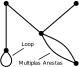
\includegraphics[width=0.28\linewidth]{secGrafos/figures/pseudograph.png}
	\end{center}
	\caption{Exemplo de pseudografo contendo 5 vértices e 6 arestas.}
	\label{fig:pseudograph}
\end{figure}

Porém, para esse trabalho não interessa o estudo de multigrafos ou pseudografos. Por isso, adotou-se uma definição alternativa para grafos, visando restringir sua aplicação, como segue:

\begin{center}
	\begin{minipage}{0.9 \linewidth}
		\textbf{Definição:} Um \textit{Grafo Simples} $G$ é uma dupla ordenada da forma $(V_G,E_G)$, composta por um conjunto não nulo e finito $V_G$ e outro conjunto finito $E_G$ de pares não ordenados de elementos \textbf{distintos} pertencentes a $V_G$.
	\end{minipage}
\end{center} 

Diz-se que um $(m,n)$ grafo $G$ é \textit{Rotulado} quando pode-se distinguir seus $m$ vértices ao nomeá-los --- algo como $v_1, v_2, \dots, v_m$. Por exemplo, os grafos da Figura~\ref{fig:graphisomorphic} são rotulados, enquanto o grafo da Figura~\ref{fig:pseudograph} não é. Quando não é dito o contrário, considera-se todo grafo como rotulado.

Dois grafos $G = (V_G, E_G)$ e $H = (V_H, E_H)$ são ditos \textit{Isomorfos} (escreve-se $G \cong H$) quando existe uma correspondência biunívoca entre os conjuntos de vértices $V_G$ e $V_H$ que preserve suas adjacências. A Figura~\ref{fig:graphisomorphic} ilustra essa situação, com a correspondência $v_i \longleftrightarrow v_i$.

\begin{figure}[H]
	\begin{center}
		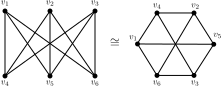
\includegraphics[width=0.6\linewidth]{secGrafos/figures/graphisomorphic.png}
	\end{center}
	\caption{Diferentes representações isomórficas de um (6, 9) grafo.}
	\label{fig:graphisomorphic}
\end{figure}

O isomorfismo é uma relação de equivalência. Fica claro que, por mais que seja útil, a representação gráfica de um grafo existe apenas como um apelo intuitivo. A forma geométrica formada pelos vértices é escolha de quem desenha. Vários são os casos em que problemas envolvendo grafos são facilmente solucionáveis apenas rearranjando a forma como se desenha --- como o caso das pontes de Köenigsberg. A resposta salta aos olhos.

\subsubsection{Subgrafos}

Diz-se que o grafo $G_1 = (V_{G_1}, E_{G_1})$ é \textit{Subgrafo} de $G = (V_G, E_G)$ se $V_{G_1} \subset V_G$ e $E_{G_1} \subset E_G$. Se $G_1$ é subgrafo de $G$, então $G$ é \textit{Supergrafo} de $G_1$. Para qualquer $V \subset V_G$, existe um \textit{Subgrafo Induzido} $\langle V \rangle$ definido por $(V, E)$, onde $E \subset E_G$ contém todas as arestas $(v_1, v_2) \in E_G$ tal que $v_1, v_2 \in V$. 
Fica claro que dois vértices em $\langle V \rangle$ são adjacentes se, e somente se, forem também adjacentes em $G$.

Pode-se \textit{remover um vértice} $v$ de um grafo $G = (V_G, E_G)$, que resulta no subgrafo induzido $G - v = \langle V_G \setminus \{v\}\rangle$. Da mesma forma, pode-se \textit{remover uma aresta} $e$ de um grafo $G = (V_G, E_G)$, resultando no grafo $G-e = (V_G, E_G \setminus \{e\})$.

\subsubsection{Caminhos}

Um \textit{Passeio} em $G$ é uma sequência finita não nula $W = v_0e_1v_1e_2v_2\dots e_kv_k$, onde seus termos são alternados entre vértices e arestas, tal que, para $1\leq i \leq k$, antes e depois de $e_i$ vem $v_{i-1}$ e $v_i$, respectivamente. Diz-se que $W$ é um passeio de $v_0$ para $v_k$, ou um $(v_0,v_k)$-passeio. Os vértices $v_0$ e $v_k$ são chamados origem e fim do passeio, respectivamente, e $v_1,v_2,\dots,v_{k-1}$ são os vértices internos. O número $k$ é o comprimento de $W$. 
Em um grafo simples, um passeio $v_0e_1v_1e_2v_2\dots e_kv_k$ é determinado suficientemente pela sequência dos vértices que o constitui $v_0v_1v_2\dots v_k$.

Se $W=v_0v_1\dots v_k$ e $W' = v_kv_{k+1}\dots v_l$ são passeios, o passeio $W^{-1} = v_kv_{k-1}\dots v_0$ é dito \textit{Passeio Reverso} de $W$ e o passeio $WW' = v_0v_1\dots v_l$ é dito \textit{Concatenação} de $W$ com $W'$. Chama-se \textit{Seção} do passeio $W$ uma subsequência $(v_i,v_j)$-seção $= v_iv_{i+1}\dots v_j$ de termos consecutivos de $W$. 

Se as arestas $e_1,e_2,\dots,e_k$ de um passeio $W$ são todas distintas --- o que sempre ocorre em grafos simples --- chama-se $W$ de \textit{Trilha}.  Se, adicionalmente, os vértices da trilha $W$ forem todos distintos, chama-se $W$ de \textit{Caminho} (também conhecido como \textit{Caminho Simples}).

\subsubsection{Conectividade}

Dois vértices $u$ e $v$ de $G$ são ditos \textit{Conectados} se existe um $(u,v)$-passeio em $G$. A conectividade induz uma relação de equivalência sobre o conjunto de vértices $V$: Há uma partição de $V$ em subconjuntos não vazios $V_1, V_2, \dots, V_\omega$ tal que dois vértices $u$ e $v$ são conectados se, e somente se, $u$ e $v$ pertencem ambos ao mesmo subconjunto $V_i$. Os subgrafos induzidos $\langle V_1\rangle, \langle V_2\rangle, \dots,\langle V_\omega\rangle$ são chamados \textit{Componentes de $G$}. Se $G$ tem exatamente uma única componente, então $G$ é dito \textit{Conectado}; e, do contrário, $G$ é dito \textit{Desconectado}. 

A Figura~\ref{fig:connectGraph} mostra dois grafos: O grafo da esquerda é conectado --- possui uma única componente $\langle \{v_1,v_2,v_3,v_4\}\rangle$; porém, o da direita não é --- pois possui duas componentes $\langle \{v_1,v_2,v_3\}\rangle$, $\langle \{v_4\}\rangle$.

\begin{figure}[H]
	\begin{center}
		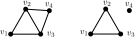
\includegraphics[width=0.6\linewidth]{secGrafos/figures/connectedGraph.png}
	\end{center}
	\caption{A esquerda um grafo conectado e, a direita, um grafo desconectado}
	\label{fig:connectGraph}
\end{figure}

\subsubsection{Grafos Completos}

Introduze-se agora uma classe especial de grafos: Um grafo é dito \textit{Completo} se possui todas as suas arestas possíveis, i.e., para cada par de vértices distintos $u, v \in V_G$, $u$ é adjacente a $v$ (vide Figura~\ref{fig:grafocompleto}).

\begin{figure}[H]
	\begin{center}
		\includegraphics[width=0.3\linewidth]{secGrafos/figures/grafocompleto.png}
	\end{center}
	\caption{Diagrama de um grafo completo com 12 vértices ($|V| = 12$).}
	\label{fig:grafocompleto}
\end{figure}

Usando combinatória, sabe-se que todo grafo completo com $n$ vértices possui ${n \choose 2}=\frac{n(n-1)}{2}$ arestas.
\\

Em particular, chama-se de \textit{$k$-Clique} um subgrafo $G'$ de $G$, com $k$ vértices, tal que $G'$ é completo, independente se seu supergrafo $G$ é ou não completo. Por exemplo, selecionando arbitrariamente quaisquer dois vértices do grafo da Figura~\ref{fig:grafocompleto}, pode-se gerar um $2$-clique induzido por estes e, caso toma-se 3 vértices, pode-se gerar um $3$-clique (veja a Figura~\ref{fig:cliques}).

\begin{minipage}{0.55 \linewidth}
	\begin{figure}[H]
		\begin{center}
			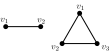
\includegraphics[width=0.74\linewidth]{secGrafos/figures/cliques.png}
		\end{center}
		\caption{(a) 2-clique e (b) 3-clique.}
		\label{fig:cliques}
	\end{figure}
\end{minipage}
\hspace{0.1cm}
\begin{minipage}{0.40 \linewidth}
	\begin{figure}[H]
		\begin{center}
			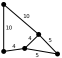
\includegraphics[width=0.485\linewidth]{secGrafos/figures/weightedGraph.png}
		\end{center}
		\caption{Grafo ponderado.}
		\label{fig:weightedGraph}
	\end{figure}
\end{minipage}

\subsubsection{Grafos Ponderados}

As arestas $e\in E$ de um grafo $G$ pode estar associadas com um número real $d(e)$, chamado de \textit{Peso da Aresta $e$} (veja a Figura~\ref{fig:weightedGraph}). Quando $G$ tem todas as suas arestas associadas com pesos, define-se $G$ como um \textit{Grafo Ponderado}. Grafos ponderados são frequentemente associados com aplicações em teoria de grafos \cite{grafosPremioElon}.

Costuma-se definir uma \textit{Função Ponderação} $d: E \longrightarrow \mathbb{R}$ para mapear o conjunto de arestas $E$ no conjunto dos números reais $\mathbb{R}$ \cite{libertiEDG}. Escreve-se $G = (V_G,\;E_G,\;d)$ como um grafo ponderado $(V_G,\; E_G)$ e função ponderação $d$.


